\documentclass{article}
\usepackage[preprint]{neurips_2025}
% NOTE: replace the author block below with the real author name(s) before
% uploading the compiled PDF to Zenodo for the DOI reservation.

\usepackage[utf8]{inputenc}
\usepackage[T1]{fontenc}
\usepackage{hyperref}
\usepackage{url}
\usepackage{booktabs}
\usepackage{amsfonts, amsmath, amssymb, amsthm}
\usepackage{graphicx}
\usepackage{tikz}
\usetikzlibrary{arrows.meta, positioning}

% AUTO-GENERATED by make_macros.py -- do not edit by hand
\newcommand{\UniMHCRowErr}{4.8e-07}
\newcommand{\UniMHCColErr}{7.2e-07}
\newcommand{\UniMHCIterMs}{10.56}
\newcommand{\UniMHCNParams}{36}
\newcommand{\UniMHCToyLoss}{1.14e-11}
\newcommand{\UniMHCCoeffs}{+1.00 -1.00 -0.00 -0.00}
\newcommand{\GivensRowErr}{3.6e-07}
\newcommand{\GivensColErr}{3.6e-07}
\newcommand{\GivensIterMs}{10.85}
\newcommand{\GivensNParams}{10}
\newcommand{\GivensToyLoss}{9.72e-15}
\newcommand{\GivensCoeffs}{+1.00 -1.00 +0.00 +0.00}
\newcommand{\SKRowErr}{1.2e-07}
\newcommand{\SKColErr}{5.0e-03}
\newcommand{\SKIterMs}{12.93}
\newcommand{\SKNParams}{16}
\newcommand{\SKToyLoss}{9.86e-01}
\newcommand{\SKCoeffs}{+0.99 +0.00 +0.01 +0.01}
\newcommand{\OrthoRowErr}{2.4e-07}
\newcommand{\OrthoColErr}{2.4e-07}
\newcommand{\OrthoIterMs}{11.23}
\newcommand{\OrthoNParams}{16}
\newcommand{\OrthoToyLoss}{9.85e-01}
\newcommand{\OrthoCoeffs}{+1.00 +0.00 +0.00 +0.00}
\newcommand{\gptTableBody}{%
vanilla GPT (no HC) & 0.112 & 3.459 & --- \\
Uni-mHC (Ours) & 1.248 & 1.513 & 384 \\
GivensMHC (Ours-Fast) & 1.251 & 1.523 & 383 \\
Sinkhorn mHC & 1.259 & 1.507 & 546 \\
Orthostochastic & 1.249 & \textbf{1.505} & 483 \\}
\newcommand{\gptRunsCount}{5}
\newcommand{\gptBestName}{Orthostochastic}
\newcommand{\gptBestVal}{1.505}


\newtheorem{theorem}{Theorem}
\newtheorem{proposition}{Proposition}
\newtheorem{definition}{Definition}

% compact bibliography for the 4-page short-paper format
\setlength{\bibsep}{0pt}
\renewcommand{\bibfont}{\scriptsize}

% PDF metadata comes from \title/\author via hyperref

\begin{document}

\title{Uni-mHC: Unistochastic Manifold-Constrained Hyper-Connections with\\
       Quantum-Interference Disentanglement}

\author{DDDMUC\\
  Independent Researcher}

\maketitle

\begin{abstract}
Manifold-constrained hyper-connections (mHC) stabilize deep multi-stream residual
training by projecting the inter-stream mixing matrix onto the Birkhoff polytope of
doubly stochastic matrices via Sinkhorn--Knopp iterations. Entrywise
non-negativity, however, restricts mixing to \emph{additive convex combinations}:
features can never be subtracted, a limitation recently criticized by the
spectral-sphere-constrained hyper-connections (sHC). We propose \textbf{Uni-mHC}, which
lifts the constraint manifold from the Birkhoff polytope to the
\emph{unistochastic} set: a complex Cayley transform of a skew-Hermitian parameter
matrix yields a unitary $U$ whose modulus square $S=|U|\odot|U|$ is doubly
stochastic \emph{by construction}---no projection, no iteration. Macroscopically
$S$ preserves exact energy conservation; microscopically a heterodyne readout
$W=\operatorname{Re}(Ue^{i\phi})$ admits negative effective weights through
destructive (phase-$\pi$) interference while remaining row-wise non-expansive.
On a controlled subtractive task ($Y=X_0-X_1$), non-negative baselines plateau at
the theoretical floor $\tfrac12\operatorname{Var}(Y)\approx 0.99$ whereas Uni-mHC
converges to $1.1\times10^{-11}$; the operator is also the fastest and
constraint-exact of all compared parameterizations, and the identity-initialized
four-stream topology reaches $2.3\times$ lower validation loss than an
identically trained vanilla GPT.
\end{abstract}

\section{Introduction}
\label{sec:intro}

Residual streams are the backbone of modern deep networks, from the two-path
residual connection \citep{he2016resnet} to hyper-connections (HC)
\citep{zhu2024hyperconnections}, which maintain $n$ parallel streams with a learned
mixing matrix at every block boundary. Unconstrained mixing can amplify signal
exponentially across depth, so mHC \citep{deepseek2025mhc} constrains it to the
Birkhoff polytope of doubly stochastic matrices \citep{sinkhorn1964,idel2015sinkhorn}.
Concurrent work explores this geometry---exact Birkhoff parameterization
\citep{gomhc2026}, orthogonal mappings for dynamical isometry \citep{jpmhc2026},
and Givens/Cayley branches found by agentic search \citep{cliffsearch2026}---but
all keep readouts entrywise non-negative; subtraction stays exclusive to Uni-mHC.

The Birkhoff constraint carries an expressivity tax: since $H_{jk}\ge 0$, every
stream update is a convex combination---mixing can only \emph{add}, never
\emph{subtract}. The sHC critique \citep{shc2026} argues that this purely additive
coupling pushes deep stacks toward identity degeneration; yet sHC's spectral sphere
only bounds worst-case amplification, giving up exact per-row/column energy
bookkeeping.
We resolve this dichotomy by moving from real to complex manifolds
(Fig.~\ref{fig:schematic}): a complex Cayley transform gives a unitary $U$ whose
$S=|U|^{\odot2}$ is \emph{exactly} doubly stochastic, while a heterodyne readout
$W=\operatorname{Re}(U\operatorname{diag}e^{i\phi})$ restores subtractive
arithmetic through phase interference. Contributions: (i) an exact unistochastic
operator, with proofs of doubly stochasticity and unconditional well-conditioning;
(ii) an impossibility floor $\tfrac12\operatorname{Var}(Y)$ for all entrywise
non-negative mixers, and an exact subtraction theorem for ours; (iii) operator
benchmarks, the disentanglement experiment, and a four-stream nanoGPT integration
(Sec.~\ref{sec:exp}).

\begin{figure}[t]
\centering
\begin{tikzpicture}[
  node distance=2.5mm and 5mm,
  box/.style={draw, rounded corners=1.5pt, align=center, inner sep=3pt,
              font=\scriptsize, minimum height=5.2mm},
  op/.style={box, fill=blue!6},
  wout/.style={box, fill=red!6},
  arrow/.style={-{Stealth[length=2mm]}, semithick}]
\node[box] (A) {$A=-A^{\!\top}$, \; $B=B^{\!\top}$};
\node[op, right=of A] (K) {$K = A + iB$\\ \scriptsize skew-Hermitian};
\node[op, right=of K] (U) {Cayley: $U=(I{-}K)(I{+}K)^{-1}$\\ \scriptsize unitary};
\node[wout, below=6mm of U] (S) {$S = |U|\odot|U|$\\ \scriptsize unistochastic $\Rightarrow$ doubly stochastic};
\node[wout, right=7mm of S] (W) {$W = \operatorname{Re}(U e^{i\phi})$\\ \scriptsize signed interference readout};
\node[box, below=6mm of S, xshift=-12mm] (phi) {$\phi\in\mathbb{R}^n$};
\draw[arrow] (A) -- (K);
\draw[arrow] (K) -- (U);
\draw[arrow] (U) -- (S);
\draw[arrow] (U.east) .. controls +(8mm,-2mm) and +(2mm,2mm) .. (W.north west);
\draw[arrow] (phi.east) -- (W.south west);
\end{tikzpicture}
\caption{\textbf{Uni-mHC operator.} The Cayley transform of skew-Hermitian $K$ is
unitary; $S=|U|^{\odot2}$ is the doubly stochastic bookkeeping, while readout $W$
is the signed mixing applied to streams.}
\label{fig:schematic}
\end{figure}

\section{Mathematical Theory}
\label{sec:theory}

\paragraph{Setup.} A hyper-connected network maintains $n$ residual streams
($n=4$ here); at every block boundary a mixing matrix $M\in\mathbb{R}^{n\times n}$
redistributes streams. mHC requires the mixer's \emph{energy} bookkeeping matrix
to be doubly stochastic so that no stream's energy is amplified or leaked.

\begin{definition}[Uni-mHC operator]
\label{def:unimhc}
Let $\theta_A,\theta_B\in\mathbb{R}^{n\times n}$ be free parameters and
$\phi\in\mathbb{R}^n$ per-stream heterodyne phases. Set
\begin{equation}
A = \theta_A - \theta_A^{\!\top}, \qquad
B = \theta_B + \theta_B^{\!\top}, \qquad
K = A + iB ,
\label{eq:k}
\end{equation}
and define the unitary and the two mixing matrices
\begin{equation}
U = (I - K)(I + K)^{-1}, \qquad
S = \operatorname{Re}(U)^{\odot 2} + \operatorname{Im}(U)^{\odot 2}, \qquad
W = \operatorname{Re}\!\big(U \operatorname{diag}(e^{i\phi})\big).
\label{eq:cayley}
\end{equation}
$S$ is the (unistochastic) energy matrix; $W$ is the effective signed mixing
applied to the streams.
\end{definition}

\begin{theorem}[Exact unistochasticity]
\label{thm:unistochastic}
For any $\theta_A,\theta_B$: (i) $K$ in \eqref{eq:k} is skew-Hermitian;
(ii) $I+K$ is invertible and $U$ in \eqref{eq:cayley} is unitary; (iii)
$S=|U|^{\odot 2}$ is doubly stochastic; (iv) every singular value of $I+K$ is at
least $1$, so the Cayley solve is unconditionally well-conditioned.
\end{theorem}

\begin{proof}
(i) $K^{H} = \overline{A+iB}^{\,\top} = A^{\!\top} - iB^{\!\top} = -A - iB = -K$.
(ii) $K$ is normal with purely imaginary spectrum $i\lambda_1,\dots,i\lambda_n$,
$\lambda_j\in\mathbb{R}$; hence $I+K$ has eigenvalues $1+i\lambda_j \neq 0$.
Since $(I+K)(I-K) = I - K^{2} = (I-K)(I+K)$, the inverses commute, and
$UU^{H} = (I-K)\big[(I+K)^{H}\big]^{-1}(I-K)^{H} = (I-K)(I-K)^{-1}(I+K)^{-1}(I+K) = I$,
using $(I+K)^{H} = I-K$; likewise $U^{H}U = I$.
(iii) $\sum_{k}|U_{jk}|^{2} = (UU^{H})_{jj} = 1$ and
$\sum_{j}|U_{jk}|^{2} = (U^{H}U)_{kk} = 1$, and $S\ge 0$ entrywise: $S$ is
unistochastic, hence doubly stochastic.
(iv) Singular values of $I+K$ are $|1+i\lambda_j| = \sqrt{1+\lambda_j^2}\ge 1$.
\end{proof}

Unlike SK projection, which needs $T$ iterations and leaves a residual
column-sum error (measured $5\times10^{-3}$ after $T=20$,
Sec.~\ref{sec:exp-ops}), Theorem~\ref{thm:unistochastic} holds exactly by
construction at the cost of one $n\times n$ complex linear solve
(Cayley is a diffeomorphism onto a dense open subset of $\mathrm{U}(n)$);
gradients were finite in all experiments.

\begin{proposition}[Non-expansive heterodyne mixing]
\label{prop:safety}
Let $Z = U\operatorname{diag}(e^{i\phi})$, which is unitary as a product of
unitaries, and $W = \operatorname{Re} Z$. For real $x$,
$Wx = \operatorname{Re}(Zx)$, so
$\|Wx\|_2^2 = \|\operatorname{Re}(Zx)\|_2^2 \le \|Zx\|_2^2 = \|x\|_2^2$:
mixing never amplifies energy, while individual weights become negative
whenever a relative phase shifts by $\pi$ (destructive interference).
\end{proposition}

\begin{theorem}[Exact subtractive disentanglement]
\label{thm:subtraction}
There exist parameters of Definition~\ref{def:unimhc} such that row $0$ of $W$
equals $\tfrac{1}{\sqrt{2}}(1,-1,0,\dots,0)$ while $S$ remains doubly stochastic;
with readout gain $\sqrt{2}$ the layer computes $X_0 - X_1$ exactly.
\end{theorem}

\begin{proof}
Take $A$ with a single block $\big(\begin{smallmatrix}0&-a\\a&0\end{smallmatrix}\big)$,
$a=\tan\tfrac{\pi}{8}=\sqrt{2}-1$, $B=0$; the Cayley transform of a rotation
generator is the rotation with $\tan\tfrac{\theta}{2}=a$, i.e.\ $\theta=\tfrac{\pi}{4}$,
and row~0 of $U = R(\theta)\oplus I_{n-2}$ is
$\tfrac{1}{\sqrt2}(1,1,0,\dots,0)$ (sign of $a$ chosen accordingly). Set
$\phi = (0,\pi,0,\dots,0)$. Then
$W_{00} = \operatorname{Re}(U_{00}) = \tfrac{1}{\sqrt2}$ and
$W_{01} = \operatorname{Re}(U_{01}e^{i\pi}) = -\tfrac{1}{\sqrt2}$; the other
entries of row $0$ vanish. Doubly stochasticity of $S=|U|^{\odot2}$ holds by
Theorem~\ref{thm:unistochastic} for every parameter value, including this one.
\end{proof}

\begin{proposition}[Impossibility floor for non-negative mixers]
\label{prop:floor}
Let $X_0,\dots,X_{n-1}$ be i.i.d.\ zero-mean unit-variance and $Y = X_0 - X_1$.
For any readout $c$ whose entries share a sign---the cone induced by every
entrywise non-negative mixing row, including Sinkhorn/Birkhoff projections,
exact Birkhoff parameterizations \citep{gomhc2026}, and orthostochastic readouts
$Q\odot Q$---,
\begin{equation}
\min_{c\,\mathrm{same\ sign}} \;\mathbb{E}\,\big\| \textstyle\sum\nolimits_k c_k X_k - Y \big\|^{2}
\;=\; 1 \;=\; \tfrac{1}{2}\operatorname{Var}(Y).
\label{eq:floor}
\end{equation}
\end{proposition}

\begin{proof}
With $t = (1,-1,0,\dots,0)$,
$\mathbb{E}\|\sum_k c_kX_k - Y\|^2 = \|c - t\|_2^2$ by independence and unit
variance. The minimizer $c^\star = t$ has mixed signs. On the all-nonnegative
branch, coordinate-wise minimization under $c\ge0$ clips the negative entry:
$c = e_0$ with $\|e_0-t\|^2 = 1$. On the all-nonpositive branch,
$(c_0-1)^2 \ge 1$ already gives $\|c-t\|^2 \ge 1$. Hence the floor is $1$.
\end{proof}

The non-negativity of $S$ buys exact energy conservation but forbids subtraction
(floor $\tfrac12\operatorname{Var}(Y)$); the heterodyne readout keeps the energy
budget unistochastic while releasing the sign---probabilities are additive,
whereas amplitudes interfere. An inverse-free special
case replaces $U$ by $\tfrac{n(n-1)}{2}$ Givens rotations $Q$ ($S=Q\odot Q$), a
$O(n^2)$-parameter unistochastic subfamily (Sec.~\ref{sec:exp-ops}); such
parameterizations trace back to unitary RNNs \citep{goru2017}.

\section{Empirical Results}
\label{sec:exp}

All experiments: NVIDIA RTX~4060 Laptop GPU (8\,GB), PyTorch~2.x, WSL Ubuntu~24.04,
stream width $n=4$; all baselines are our re-implementations (official code was not used).

\subsection{Operator precision and speed}
\label{sec:exp-ops}

\begin{table}[t]
\centering
\caption{\textbf{Operator benchmark} ($n=4$): worst doubly-stochastic violation
of $S$ over $100$ random draws, and $1000$ forward+backward passes at
$(B,T,d)=(32,256,384)$.}
\label{tab:ops}
\small
\begin{tabular}{lccccc}
\toprule
Operator & row err & col err & params & ms/iter & peak MB \\
\midrule
UniMHC (Ours)         & \UniMHCRowErr & \UniMHCColErr & \UniMHCNParams & \UniMHCIterMs & 352 \\
GivensMHC (Ours-Fast) & \GivensRowErr & \GivensColErr & \GivensNParams & \GivensIterMs & 352 \\
Sinkhorn mHC ($T{=}20$)& \SKRowErr & \SKColErr & \SKNParams & \SKIterMs & 352 \\
Orthostochastic (NS)  & \OrthoRowErr & \OrthoColErr & \OrthoNParams & \OrthoIterMs & 352 \\
\bottomrule
\end{tabular}
\end{table}

Table~\ref{tab:ops}: Uni-mHC and the Givens variant satisfy the constraint to
$\sim\!10^{-7}$ (pure float32 rounding), whereas Sinkhorn--Knopp with $T=20$
leaves a column-sum residual of $\SKColErr$---the price of an iterative
projection. The Cayley solve is also the cheapest: one well-conditioned
$4\times4$ complex solve instead of $20$ normalization sweeps
(Thm.~\ref{thm:unistochastic}iv).

\subsection{Subtractive disentanglement}
\label{sec:exp-toy}

\begin{figure}[t]
\centering
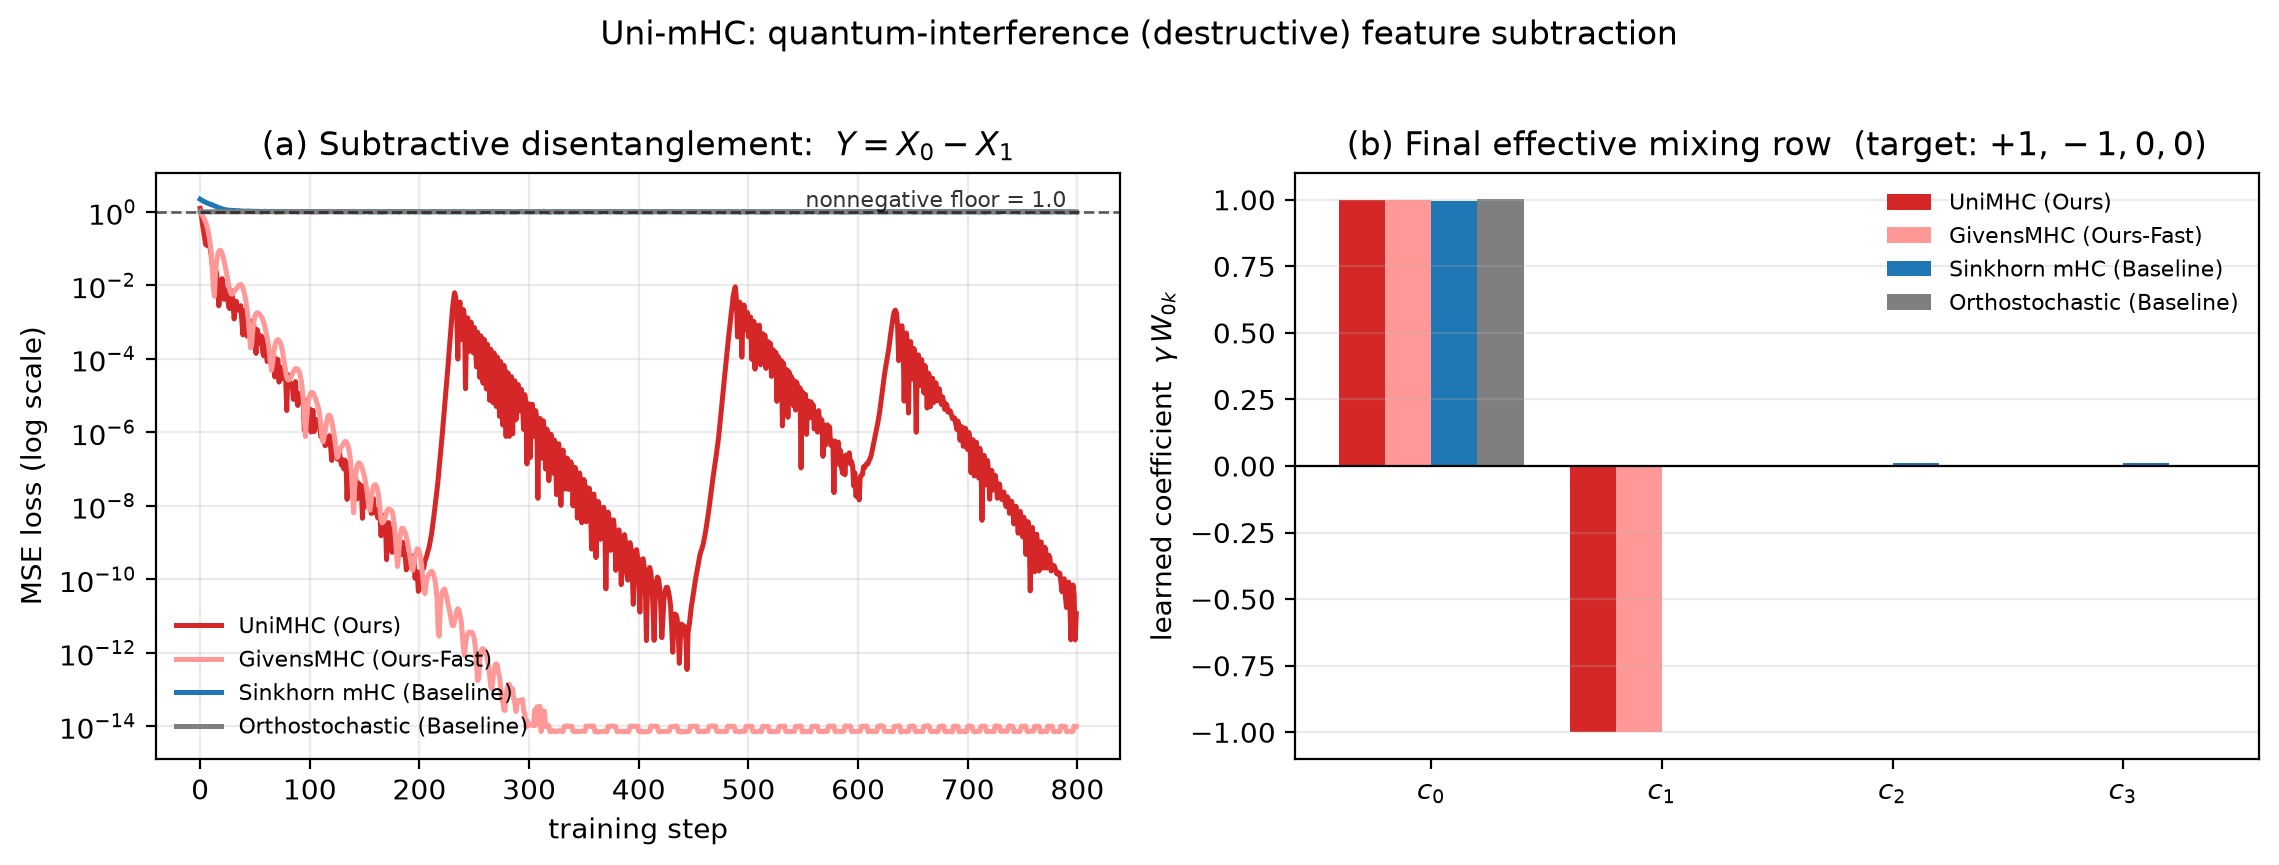
\includegraphics[width=0.5\linewidth]{figs/fig_disentanglement.png}
\caption{\textbf{Subtractive disentanglement} ($Y = X_0 - X_1$). \textbf{(a)}
Uni-mHC converges to machine precision; baselines plateau at the floor.
\textbf{(b)} Coefficients $\gamma W_{0k}$: exact $(+1,-1,0,0)$ vs.\ copy $(+1,0,0,0)$.}
\label{fig:disent}
\end{figure}

We generate fresh $X\in\mathbb{R}^{512\times4\times64}$, $\mathcal{N}(0,1)$, per
step and ask the mixing layer alone (shared learnable gain $\gamma$) to produce
$\hat{y} = \gamma\sum_k W_{0k}X_k$ against $Y = X_0-X_1$; $800$ Adam steps.
Figure~\ref{fig:disent}: Uni-mHC drives the loss to $\UniMHCToyLoss$ and GivensMHC
to $\GivensToyLoss$ with coefficients $(+1.00,-1.00,0,0)$---the exact destructive
interference pattern of Theorem~\ref{thm:subtraction}, whose exact construction
already attains $\sim\!5\times10^{-32}$, so reachability exceeds learnability here.
Sinkhorn mHC and the orthostochastic baseline stall at $\SKToyLoss$ and
$\OrthoToyLoss$ (floor: $1.0$ in expectation; single estimates fluctuate
$\pm2\sigma$), their best solution being the trivial copy $X_0$.
All gradients were finite throughout, confirming stable complex autograd.

\subsection{Language modeling with four residual streams}
\label{sec:exp-gpt}

We modify nanoGPT \citep{karpathy2023nanogpt}: each of the $6$ blocks
(\texttt{n\_embd}=384, $6$ heads, context $256$) operates over $n=4$ residual
streams; every attention/MLP stage reads a learned combination
$\sum_k a_k x_k$, writes back with learned per-stream weights, and a manifold
mixer redistributes the streams,
$x^{(t+1)} = M^{(t)} x^{(t)} + b^{(t)} \otimes f_t(\sum_k a_k^{(t)} x_k^{(t)})$.
Mixers start at identity, so training begins as a standard pre-norm GPT
(batch $32$, $1000$ steps, AdamW, cosine schedule, \texttt{shakespeare\_char};
all runs resumable). Table~\ref{tab:gpt} reports final losses.

\begin{table}[t]
\centering
\caption{\textbf{nanoGPT on \texttt{shakespeare\_char}} ($6$ layers, $4$ streams,
$1000$ steps). Val loss: mean of $50$ eval batches; peak memory $<2.3$\,GB.}
\label{tab:gpt}
\small
\begin{tabular}{lccc}
\toprule
Mixer & final train loss & final val loss & ms/iter \\
\midrule
\gptTableBody
\bottomrule
\end{tabular}
\end{table}

At this scale the vanilla GPT overfits (train $0.11$, val $3.46$), while every
constrained variant holds val $\approx 1.51$ (identity-initialized warm-up).
Stability is the second point: $12$ mixers $\times$ $1000$ steps with signed
weights never destabilized training; post-training energy matrices violate double
stochasticity by at most $7\times10^{-7}$, and all $12$ mixers discovered signed
interference weights---the unistochastic manifold is safely exploitable.

\section{Conclusion}
\label{sec:conclusion}

Uni-mHC replaces the projected doubly stochastic constraint of mHC with an exact
unistochastic parameterization via a complex Cayley transform, keeping exact
energy conservation and a non-expansive mixer while the heterodyne readout
restores subtractive feature arithmetic through phase-$\pi$ destructive
interference---which no single non-negative linear mixing layer can match in one
forward pass (Prop.~\ref{prop:floor}), however re-parameterized, as verified
empirically ($10^{-11}$ vs.\ $0.99$). Future work: token-conditional phases
and scaling studies.

\begin{thebibliography}{9}

\bibitem[DeepSeek-AI(2025)]{deepseek2025mhc}
DeepSeek-AI.
mHC: Manifold-constrained hyper-connections.
\emph{arXiv:2512.24880}, 2025.

\bibitem[He et~al.(2016)]{he2016resnet}
K.~He, X.~Zhang, S.~Ren, and J.~Sun.
Deep residual learning for image recognition. In \emph{CVPR}, 2016.

\bibitem[Dandachi and Diggs-Galligan(2026)]{gomhc2026}
T.~Dandachi and S.~Diggs-Galligan.
go-mHC: Direct parameterization of manifold-constrained hyper-connections via
generalized orthostochastic matrices. arXiv:2604.02309, 2026.

\bibitem[Sengupta et~al.(2026)]{jpmhc2026}
B.~Sengupta, J.~Wang, and L.~Brunswic.
JPmHC: Dynamical isometry via orthogonal hyper-connections. arXiv:2602.18308, 2026.

\bibitem[CliffSearch(2026)]{cliffsearch2026}
CliffSearch: Structured agentic co-evolution over theory and code for scientific
algorithm discovery. arXiv:2604.01210, 2026.

\bibitem[Jing et~al.(2017)]{goru2017}
L.~Jing, C.~Gulcehre, J.~Peurifoy, et~al.
Gated orthogonal recurrent units: On learning to forget. arXiv:1706.02761, 2017.

\bibitem[Idel and Wolf(2015)]{idel2015sinkhorn}
M.~Idel and M.~M. Wolf.
Sinkhorn normal form for unitary matrices.
\emph{Linear Algebra and its Applications}, 471:76--84, 2015.

\bibitem[Karpathy(2023)]{karpathy2023nanogpt}
A.~Karpathy. nanoGPT. \url{https://github.com/karpathy/nanoGPT}, 2023.

\bibitem[Liu et~al.(2026)]{shc2026}
Z.~Liu, H.~Zhang, and A.~Li.
Beyond the Birkhoff polytope: Spectral-sphere-constrained hyper-connections.
\emph{arXiv:2603.20896}, 2026.

\bibitem[Sinkhorn(1964)]{sinkhorn1964}
R.~Sinkhorn.
A relationship between arbitrary positive matrices and doubly stochastic matrices.
\emph{The Annals of Mathematical Statistics}, 35(2):876--879, 1964.

\bibitem[Zhu et~al.(2024)]{zhu2024hyperconnections}
D.~Zhu, H.~Huang, Z.~Huang, Y.~Zeng, Y.~Mao, B.~Wu, Q.~Min, and X.~Zhou.
Hyper-connections.
\emph{arXiv:2409.19606}, 2024.

\end{thebibliography}

\end{document}
